\documentclass[12pt,a4paper]{report}
\usepackage[utf8]{vietnam}
\usepackage{amsmath}
\usepackage{amsfonts}
\usepackage{amssymb}
\usepackage{makeidx}
\usepackage{graphicx}
\usepackage{fancybox}
\usepackage[left=3.50cm, right=2.00cm, top=3.50cm, bottom=3.00cm]{geometry}
\usepackage{scrextend}
\changefontsizes{13pt}
\usepackage{fancyhdr}
\pagestyle{fancy}
\lhead{\textit{Kiểm soát phản hồi trạng thái tối ưu}}
\chead{}
\rhead{\textit{GVHD: PGS Đỗ Đức Thuận}}
\lfoot{\textit{SVTH: Hoàng Thanh Lưu}}
\cfoot{\thepage}
\rfoot{\textit{Toán Tin K61}}
\renewcommand{\headrulewidth}{0.4pt}
\renewcommand{\footrulewidth}{0.4pt}
\begin{document}
	\thisfancypage{%đóng khung trang này
	\setlength{\fboxsep}{0pt}% 8pt là độ dày của đường viền
	\fbox}{} % phần nội dung sau là tương tự như đã làm
\thispagestyle{empty}
\begin{center}
	\vspace*{0.4cm}
	\fontsize{14}{12}
	\textbf{TRƯỜNG ĐẠI HỌC BÁCH KHOA HÀ NỘI}\\
	\textbf{VIỆN TOÁN ỨNG DỤNG VÀ TIN HỌC}\\
	\textbf{------ o0o ------}
\end{center}
\vspace*{0.8cm}
\begin{center}
	
\includegraphics[scale=.5]{bk.png}
\end{center}
\vspace*{0.8cm}
\begin{center}
	\fontsize{20}{18}
	\textbf{KIỂM SOÁT PHẢN HỒI TRẠNG THÁI TỐI ƯU}\\
	\vspace*{0.8cm}
	\fontsize{18}{16}
	\textbf{ĐỒ ÁN III}
\end{center}
\vspace*{0.7cm}
\begin{center}
	\fontsize{14}{16}
	\begin{tabular}{ll}
		
		\textbf{Giảng viên hướng dẫn:} & \textbf{PGS.TS Đỗ Đức Thuận} \\ 
		\textbf{Sinh viên thực hiện:} & \textbf{Hoàng Thanh Lưu} \\ 
		\textbf{Lớp:}  & \textbf{Toán Tin K61} \\ 
	\end{tabular} \\
	\vspace*{2.5cm}
	\fontsize{14}{16}
	\textbf{Hà Nội - 6/2020}
\end{center}
	\newpage
	\thispagestyle{empty}
	\begin{center}
		\fontsize{14}{16}	
		\textbf{NHẬN XÉT CỦA GIẢNG VIÊN HƯỚNG DẪN}
		\vspace*{0.7cm}
	\end{center}
	\textbf{1. Mục đích và nội dung của đồ án.}\\\\
	.............................................................................................................................\\.............................................................................................................................\\.............................................................................................................................\\.............................................................................................................................\\.............................................................................................................................\\\\
	\textbf{2. Kết quả đạt được.}\\\\
	.............................................................................................................................\\.............................................................................................................................\\.............................................................................................................................\\.............................................................................................................................\\.............................................................................................................................\\\\
	\textbf{3. Ý thức làm việc của sinh viên.}\\\\
	.............................................................................................................................\\.............................................................................................................................\\.............................................................................................................................\\.............................................................................................................................\\.............................................................................................................................\\\\
	
	\begin{flushright}
		\begin{tabular}{cccc}
			&   \textit{ Hà Nội ngày $\quad$ tháng  6 năm 2020} && \\ 
			&    Giảng viên hướng dẫn && \\ 
			&    \textit{(Ký và ghi rõ họ tên)} && \\ 
		\end{tabular} 
	\end{flushright}
		\tableofcontents
	\chapter{Các khái niệm cơ bản}
	
	\chapter{Một số vấn đề về  bài toán điều khiển tối ưu}
	\section{Nguyên lý cực đại Pontryagin}
	\subsubsection{Xét hệ điều khiển} \begin{equation}
		\dot{x} = f(x, u), f: \mathbb{R}^n \times \mathbb{R}^m \to \mathbb{R}^n, f = (f_1, ..., f_n)^T, f_i: \mathbb{R}^n \times \mathbb{R}^m \to \mathbb{R}
	\end{equation}
	Một số lưu ý
	\begin{itemize}
		\item $x(0) = 0 \in \mathbb{R}^n$ \\ $x(t_1) = x_1$ cho trước thì bài toán là bài toán cố định \\ $x(t_1) = x_1$ không cho trước thì bài toán là bài toán tự do
		\item $x \in$ $\Delta$ là lớp điều khiển chấp nhận được, $x(t) \in \Omega \subset \mathbb{R}^m$
		\item Hàm tối ưu \begin{equation}
			C(x) = \int_{0}^{t_1}f_0(x(t), u(t))dt \to \min \nonumber
		\end{equation}
	\end{itemize}
	\subsubsection{Xây dựng hàm Hamilton}
	\begin{equation}
		H(x, u, \varphi) = \varphi_0f_0(x, u) + \varphi_1f_1(x, u) + \cdots + \varphi_nf_n(x, u)
	\end{equation} trong đó $\varphi_0, \varphi_1, ..., \varphi_n \in \mathbb{R}$
	\subsubsection{Viết lại hàm Haminton}
	\begin{eqnarray}
		H(x, u, \varphi) = \varphi_0f_0(x, u) + \langle \varphi, f \rangle = \varphi_0f_0(x, u) + \varphi^Tf 
	\end{eqnarray} trong đó $\varphi = (\varphi_1,...,\varphi_n)^T$.
	
	\subsubsection{Định lý PMP} Giả sử $u^*$ là điều khiển tối ưu tương ứng với quỹ đạo trạng thái tối ưu $x^*$. Khi đó tồn tại hàm $\varphi^*(t) = \big(\varphi_1^*(t),..., \varphi_n^*(t)\big)^T$ và hệ số $\varphi_0^*$ thỏa mãn:
	\begin{itemize}
		\item[\textbf{(a)}] $\dot{x}^* = f(x^*, u^*)$
		\item[\textbf{(b)}] $\dot{\varphi}_i^* = \dfrac{-\partial H}{\partial x_i} = -\varphi_0^*\dfrac{\partial f_0}{\partial x_i} - \varphi_1^*\dfrac{\partial f_1}{\partial x_i} - ... - \varphi_n^*\dfrac{\partial f_n}{\partial x_i}$
		\item[\textbf{(c)}]$\varphi_0^*$ là không dương và $$H(x^*, u^*, \varphi^*) = \max_{v\in \Omega}H(x^*, v, \varphi^*) = M(x^*, \varphi^*)$$
	\end{itemize} Hơn nữa $M(x^*(t), \varphi^*(t))$ là hằng số với $0 \leq t \leq t^*$. \subsubsection{Chú ý} Nếu các hàm $f_0, f$ khả vi liên tục thì không mất tổng quát ta có thể giả sử $\varphi_0^* = -1$. Đối với bài toán tự do ($x^*(t^*) = x_1$ không cho trước) thì ta có thêm điều kiện hoành $\varphi^*(t^*) = 0$.

\section{Nguyên lý quy hoạch động Bellman}
\subsection{Phương trình Hamilton-Jacobi-Bellman}
\textbf{Xét hệ điều khiển} 
\begin{eqnarray}
	\dot{x}(t) &=& f(x(t), u(t)) \nonumber \\ x(t_0) &=& x_0 \nonumber
\end{eqnarray} Hàm mục tiêu $$C(u) = \int_{t_0}^{T}f_0(x(t), u(t))dt \to \min$$
Giả sử $V(x_1, t_1)$ là giá trị hàm mục tiêu tối ưu xuất phát từ $t_1$ với trạng thái ban đầu $x(t_1) = x_1$, tức là giá trị của hàm $$\int_{t_1}^{T}f_0(x(t), u(t))dt \to \min$$ Từ nguyên lý quy hoạch động ta có phương trình đối với hàm $V(x, T)$ \begin{equation}
	\dfrac{\partial}{\partial t}V(x, t) = - \min\big\{\nabla_xV(x,t)f(x, w) + f_0(x, w)\big\}
\end{equation} 
Điều khiển tối ưu $u^*$ là giá trị $w_{\min}$ giải phương trình này. \\\\ Trong trường hợp hàm mục tiêu có chi trả trạng thái cuối cùng $$C(u) = G(x(t)) + \int_{t_0}^{T}f_0(x(t), u(t))dt$$ thì ta có điều khiển $V(x, T) = G(x(t))$, nếu $G(x(t)) = 0$ thì ta có $V(x, T) = 0$.\\\\ Phương trình (2.4) được gọi là phương trình Hamilton-Jacobi-Bellman (HJB).
\subsection{Phương trình Riccati}
\textbf{Xét hệ điều khiển}
\begin{eqnarray}
	\dot{x}(t) &=& Ax(t) + Bu(t) \nonumber\\ x(0) &=& 0, \quad A \in \mathbb{R}^{n\times n}, B \in \mathbb{R}^{n\times m} \nonumber
\end{eqnarray} Hàm mục tiêu $$C(u) = \dfrac{1}{2}x(T)^TSx(T) + \dfrac{1}{2}\int_{0}^{T}\Big[x(t)^TQx(t) + u(t)^TRu(t)\Big]dt$$ trong đó $Q, S \in \mathbb{R}^{n\times n}$ là các ma trận xác định không âm và $R \in \mathbb{R}^{m\times m}$ là ma trận xác định dương.\\\\ Giải phương trình Hamilton-Jacobi-Bellman cho bài toán này, ta tìm được $$u^*(x, t) = -R^{-1}B^T\nabla_xV(x, t)$$ trong đó $V(x, t)$ là nghiệm của phương trình
	%%%%%%%%%%%%%%%%%%%%%%%%%%%%%%%%%
	\chapter{Kiểm soát phản hồi trạng thái tối ưu}
	\section{Nguyên tắc tối ưu}
	Xem xét vấn đề kiểm soát tối ưu sau đây với thời gian cuối cố định $t_b$:\\\\Tìm một điều khiển chấp nhận được $u$: $[t_a, t_b] \to \Omega \subseteq \mathbb{R}^m$ với các ràng buộc \begin{eqnarray}
		x(t_a) &=& x_a \nonumber \\ \dot{x}(t) &=& f(x(t), u(t), t) \qquad \text{ với } t \in [t_a, t_b] \nonumber \\ x(t_b)&\in& S \subseteq \mathbb{R}^n \nonumber
	\end{eqnarray} sao cho hàm mục tiêu đạt giá trị nhỏ nhất. $$J(u) = K(x(t_b)) + \int_{t_a}^{t_b}L(x(t),u(t), t)dt$$
	Giả sử rằng chúng ta đã tìm thấy giải pháp tối ưu toàn cục duy nhất với quỹ đạo điều khiển tối ưu $u_0$: $[t_a, t_b] \to \mathbb{R}^m$ và quỹ đạo trạng thái tối ưu tương ứng $x_0$: $[t_a, t_b] \to \mathbb{R}^n$ thỏa mãn $x_0 (t_a) = x_a$ và $x_0(t_b) \in S$.
	\\\\Bây giờ, chọn một thời gian tùy ý $\tau \in(t_a, t_b)$ và chia đôi vấn đề kiểm soát tối ưu ban đầu thành một vấn đề kiểm soát tối ưu trước đó trong khoảng thời gian $[t_a,\tau]$ và một vấn đề tối ưu thành công trong khoảng thời gian $[\tau, t_b]$.\\\\Vấn đề kiểm soát tối ưu tiền đề là:\\Tìm một điều khiển được chấp nhận $u$: $[t_a, \tau] \to \Omega$, sao cho hệ thống động $$\dot{x}(t) = f(x(t),u(t),t)$$ được chuyển từ trạng thái ban đầu $$x(t_a) = x_a$$ đến trạng thái cố định cuối cùng $$x(\tau) = x^0(\tau)$$ tại thời điểm cuối cùng cố định $\tau$ và như vậy có hàm chi phí $$J(u) = \int_{t_a}^{\tau}L(x(t),u(t),t)dt$$ là nhỏ nhất.\\\\Vấn đề kiểm soát tối ưu thành công là:\\
	Tìm một điều khiển được chấp nhận $u$: $[\tau, t_b] \to \Omega$, sao cho hệ thống động $$\dot{x}(t) = f(x(t),u(t),t)$$ 
	được chuyển từ trạng thái ban đầu nhất định $$x(\tau) = x^0(\tau)$$ đến trạng thái cuối cùng $$x(t_b) \in S$$ tại thời gian cuối cùng cố định $t_b$ và như vậy hàm chi phí $$J(u) = K(x(t_b)) + \int_{\tau}^{t_b}L(x(t),u(t),t)dt$$ là nhỏ nhất.\\\\
	\textbf{Định lý: Nguyên tắc tối ưu}
	\begin{itemize}
		\item[\textbf{1)}] Giải pháp tối ưu cho bài toán điều khiển tối ưu thành công trùng khớp với phần thành công của giải pháp tối ưu của bài toán ban đầu.
		\item[\textbf{2)}] Giải pháp tối ưu cho vấn đề kiểm soát tối ưu tiền đề trùng khớp với phần tiền đề của giải pháp tối ưu cho vấn đề ban đầu. 
	\end{itemize}
	\textbf{Chứng minh}
	\begin{itemize}
		\item[\textbf{1)}] Mặt khác, kết hợp giải pháp tối ưu của vấn đề kiểm soát tối ưu thành công với phần tiền đề của giải pháp cho vấn đề kiểm soát tối ưu ban đầu sẽ mang lại giải pháp tốt hơn cho vấn đề sau.
		\item[\textbf{2)}] Mặt khác, kết hợp giải pháp tối ưu của vấn đề kiểm soát tối ưu tiền đề với phần thành công của giải pháp cho vấn đề kiểm soát tối ưu ban đầu sẽ mang lại giải pháp tốt hơn cho vấn đề sau.
	\end{itemize}
	Về mặt khái niệm, chúng ta có thể giải quyết vấn đề điều khiển tối ưu thành công cho bất kỳ trạng thái ban đầu tùy ý $x\in \mathbb{R}^n$ tại thời điểm ban đầu $\tau$, thay vì chỉ cho giá trị cố định $x_0(\tau)$. Hơn nữa, chúng ta có thể lặp lại quá trình này trong một thời gian ban đầu tùy ý $t \in [t_a, t_b]$, thay vì chỉ cho giá trị được chọn $\tau$ ban đầu. Chỉ tập trung vào giá trị tối ưu của hàm chi phí trong tất cả các trường hợp này mang lại gọi là hàm chi phí tối ưu $$T(x,t) = \min_{u(.)} \bigg\{K(x(t_b)) + \int_{t}^{t_b}L(x(t),u(t),t)dt \big | x(t) = x \bigg\}$$
	\textbf{Bổ đề}
	\begin{enumerate}
		\item[\textbf{3)}] Giải pháp tối ưu cho vấn đề kiểm soát tối ưu tiền đề với một
		trạng thái cuối cùng tự do tại thời điểm cuối cùng cố định $\tau$ và với giá trị hàm $$J = T(x(\tau), \tau) + \int_{t_a}^{\tau}L(x(t), u(t), t)dt$$ trùng với phần tiền đề của giải pháp tối ưu cho vấn đề kiểm soát tối ưu ban đầu.
		\item[\textbf{4)}] Vector chi phí tối ưu $\lambda^0(\tau)$ tương ứng với độ dốc của hàm chi phí tối ưu để đi (cost-to-gofunction), tức là, $$\lambda^0(\tau) = \nabla _xT(x^0(\tau), \tau) \text{ với tất cả } \tau \in [t_a, t_b]$$ với điều kiện $T(x, \tau) $ là liên tục khác biệt đối với $x$ tại $x^0(\tau)$
	\end{enumerate}
	\section{Học thuyết Hamilton-Jacobi-Bellman}
	\subsection{Điều kiện đủ cho giải pháp tối ưu}
	Xem xét công thức thông thường của một vấn đề kiểm soát tối ưu với trạng thái cuối cùng không xác định tại thời điểm cuối cùng cố định: \\\\ Tìm một điều khiển liên tục từng phần $u : [t_a, t_b] \to \Omega$ sao cho hệ động lực $$\dot{x}(t) = f(x(t), u(t), t)$$ được chuyển từ trạng thái ban đầu $x(t_a) = x_a$ sang trạng thái cuối cùng tùy ý tại thời điểm cuối cùng cố định và sao cho hàm chi phí $$J(u) = K(x(t_b)) + \int_{t_a}^{t_b}L(x(t), u(t), t)dt$$ đạt min.\\\\
	Xây dựng hàm Halminton với $\lambda_0^0 = 1$ $$H(x, u \lambda, t) = L(x, u, t) + \lambda^Tf(x, u, t)$$
	Xét tập hợp $n + 1$ chiều $Z = X \times [a, b] \subseteq \mathbb{R}^n \times \mathbb{R}$, trong đó $X$ là tập con (hy vọng rất lớn) của không gian trạng thái $\mathbb{R}^n$ với bên trong không trống và $[a, b]$ là tập hợp con của trục thời gian chứa ít nhất khoảng $[t_a, t_b]$, như trong Hình 2.1.
	\begin{figure}[h]
		\centering
	  	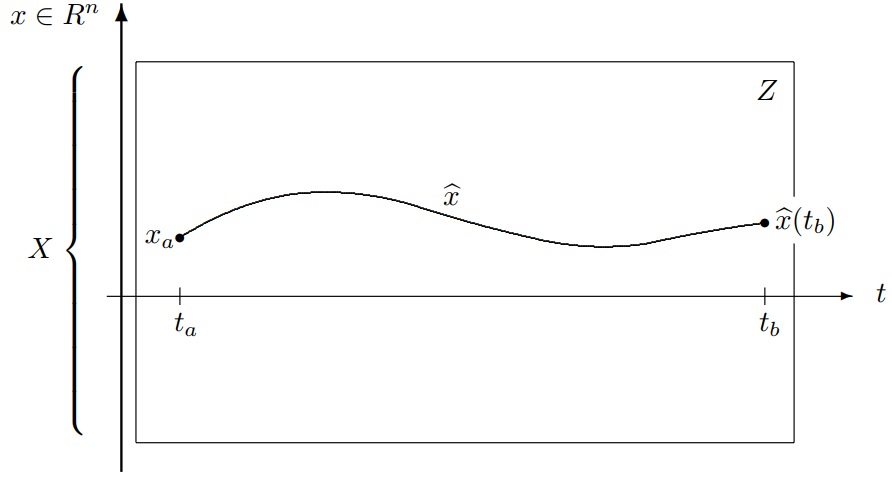
\includegraphics[scale=.6]{hinh1ct.png}
		\caption{Ví dụ quỹ đạo trạng thái $\hat{x}(.)$ không rời X}
	\end{figure}\\\\
	Chúng ta hãy xem xét các điều khiển được chấp nhận tùy ý $\hat{u}: [t_a, t_b] \to \Omega$ tạo ra các quỹ đạo trạng thái tương ứng $\hat{x}: [t_a, t_b] \to \Omega$ bắt đầu từ $x(t_a) = x_a$. Chúng ta chủ yếu quan tâm đến các quỹ đạo không rời khỏi tập $Z$, tức là thỏa mãn $x(t) \in X$ cho tất cả $t \in [t_a, t_b]$. \\\\
	Với các giả thuyết sau đây, các điều kiện đủ cho sự tối ưu toàn cục của một giải pháp cho một vấn đề điều khiển tối ưu có thể được nêu trong Định lý Hamilton-Bellman-Jacobi dưới đây.\\\\
	\textbf{Giải thuyết}
	\begin{enumerate}
		\item[\textbf{a)}] Đặt $\hat{u}: [t_a, t_b] \to \Omega$ là một điều khiển được chấp nhận tạo ra quỹ đạo trạng thái $\hat{x}: [t_a, t_b] \to \mathbb{R}^n$ với $\hat{x}(t_a) = x_a$ và $\hat{x}(.) \in Z.$
		\item [\textbf{b)}] Với tất cả $(x, t) \in Z$ và tất cả $\lambda \in \mathbb{R}^n$, để hàm Hamilton $H(x, \omega, \lambda, t) = L(x, \omega, t) + \lambda^Tf(x, \omega, t)$ có một giá trị nhỏ nhất toàn cục với $\omega \in \Omega$ tại $$\omega = \tilde{u}(x, \lambda, t) \in \Omega $$
		\item[\textbf{c)}] Đặt $T(x, t): Z \to \mathbb{R}$ là một hàm phân biệt liên tục thỏa mãn phương trình vi phân riêng phần Hamilton-Jacobi-Bellman $$\frac{\partial T(x, t)}{\partial t} + H\bigg[x, \tilde{u}\big(x, \nabla_xT(x, t), t\big), \nabla_xT(x, t), t\bigg] = 0$$ với điều kiện biên $$T(x, t_b) = K(x)$$ với tất cả $(x, t_b) \in Z$.
	\end{enumerate}
		\textit{Nhận xét:}
		\begin{itemize}
			\item Hàm $\hat{u}$ được gọi là điều khiển H thu nhỏ.
			\item Khigiar thuyết b được thỏa mãn, hàm Hamilton H được gọi là bình thường. 
		\end{itemize}
		\textbf{Định lý Hamilton-Jacobi-Bellman} \\\\ Nếu các giả thuyết a, b, và c được thỏa mãn và nếu nếu quỹ đạo điều khiển $\hat{u}(.)$ và quỹ đạo trạng thái $\hat{x}(.)$ được tạo bởi $\hat{u}(.)$ có liên quan thông qua $$\hat{u}(t) = \tilde{u}\big(\hat{x}(t), \nabla_xT(\hat{x}(t), t), t\big), $$ 
		thì giải pháp $\hat{u}, \hat{x}$ là tối ưu đối với tất cả các quỹ đạo trạng thái x được tạo bởi một quỹ đạo kiểm soát được chấp nhận $u$, không rời $X$. Hơn nữa, $T(x, t)$ là hàm chi phí tối ưu để đi (cost-to-go function).
		\\\\
		\textbf{Bổ đề} \\\\ Nếu $Z = \mathbb{R}^n \times [t_a, t_b]$ thì giải pháp $\hat{u}, \hat{x}$ là tối ưu toàn cục.
		\subsection{Luận điểm hợp lý về lý thuyết HJB}
		Chúng ta có các sự kiện sau đây:
		\begin{enumerate}
			\item [\textbf{1)}] Nếu hàm Hamilton H bình thường, chúng ta có duy nhất sau
			H-tối thiểu hóa điều khiển tối ưu: $$u^o(t) = \tilde{u}\big(x^o(t), \lambda^o(t), t\big)$$ 
			\item [\textbf{2)}] Hàm chi phí tối ưu $T(x, t)$ rõ ràng phải thỏa mãn điều kiện biên $$T(x, t_b) = K(x)$$ vì tại thời điểm cuối cùng $t_b$, giá trị hàm giá chỉ bảo gồm trạng thái cuối cùng $K(x)$.\item[\textbf{3)}] Nguyên lý tối ưu đã chỉ ra rằng chi phí tối ưu $\lambda^o(t)$ tương ứng với độ dốc của hàm chi phí tối ưu, $$\lambda^o(t) = \nabla_xT(x^o(t),t), $$ bất cứ đâu $T(x^o(t), t)$ liên tục khác biệt đối với x tại $x = x^o(t)$.
			\item [\textbf{4)}] Cùng với một quỹ đạo được chấp nhận tùy ý $u(.)$,$x(.)$, tương ứng
			hàm chi phí tối ưu $$J(x(t), t) = K(x(t_b)) + \int_{t}^{t_b}L(x(t), u(t), t)dt$$ tiến hóa theo phương trình vi phân sau: $$\frac{dJ}{dt} = \frac{\partial J}{\partial x}\dot{x} + \frac{\partial J}{\partial t} = \lambda^Tf(x, u, t) + \frac{\partial J}{\partial t} = -L(x, u, t)$$ Vì thế, $$\frac{\partial J}{\partial t} = -\lambda^Tf(x, u, t) - L(x, u, t) = -H(x, u, \lambda, t)$$ Điều này tương ứng với phương trình vi phân từng phần của hàm chi phí tối ưu $T(x, t)$, ngoại trừ luật điều khiển tối ưu chưa được áp dụng vào. 
		\end{enumerate}
	\subsection{Vấn đề điều chỉnh LQ}
	\textit{Báo cáo vấn đề điều khiển tối ưu}\\
	Tìm một luật điều khiển phản hồi trạng thái tối ưu $u$: $\mathbb{R}^n \times [t_a, t_b] \to \mathbb{R}^m$, sao cho hệ động lực tuyến tính $$\dot{x}(t)=A(t)x(t) + B(t)u(t)$$ được chuyển từ trạng thái ban đầu đã cho $x(t_a) = x_a$ sang trạng thái cuối cùng tùy ý tại  thời gian cuối cùng cố định $t_b$ sao cho hàm chi phí bậc hai
	\begin{eqnarray}
		J(u) =  \frac{1}{2}x^T(t_b)Fx(t_b) + \int_{t_a}^{t_b}\Big(\frac{1}{2}x^T(t)Q(t)x(t) + x^T(t)N(t)u(t) + \frac{1}{2}u^T(t)R(t)u(t)\Big)dt \nonumber
	\end{eqnarray} đạt min, trong đó $R(t)$ là ma trận đối xứng xác định dương và $F, Q$ và $\begin{bmatrix}
		Q(t)&N(t)\\N^T(t)&R(t)
	\end{bmatrix}$ là đối xứng và nửa xác định dương.\\\\
	\textit{Phân tích vấn đề}
	\\Xây dựng hàm Hamilton $$H = \frac{1}{2}x^TQx + x^TNu + \frac{1}{2}u^TRu + \lambda^TAx + \lambda^TBu$$ có điều khiển H-tối thiểu sau đây: $$u = -R^{-1}[B^T\lambda + N^Tx] = -R^{-1}[B^T\nabla_xT + N^Tx]$$ Do đó, phương trình vi phân từng phần Hamilton-Jacobi-Bellman là
	\begin{eqnarray}
		0 &=& \frac{\partial T}{\partial t} + H(x, \tilde{u}(x, \nabla_xT,t),\nabla_xT,t) \nonumber \\ &=& \frac{\partial T}{\partial t} + \frac{1}{2}\Big(x^TQx-x^TNR^{-1}N^Tx-\nabla_xT^TBR^{-1}B^T\nabla_xT \nonumber \\ &+& \nabla_xT^T[A-BR^{-1}N^T]x+x^T[A-BR^{-1}N^T]^T\nabla_xT\Big) \nonumber
	\end{eqnarray} với điều kiện biên $$T(x, t_b) = \frac{1}{2}x^TFx.$$
	Rõ ràng, một giả định cho hàm chi phí tối ưu $T(x, t)$ là bậc hai trong $x$ nên hoạt động. Điều này dẫn đến một phương trình vi phân từng phần trong đó tất cả các số hạng là bậc hai theo x.\textit{\textbf{(...)}} $$T(x, t) = \frac{1}{2}x^TK(t)x$$ dẫn đến $$\nabla_xT(x, t) = K(t)x \text{ và } \frac{\partial T(x, t)}{\partial t} = \frac{1}{2}x^T \dot{K}(t)x$$ Dạng cuối cùng sau đây của phương trình vi phân từng phần Hamilton-Jacobi-Bellman thu được:
	\begin{eqnarray}
		\frac{1}{2}x^T \Big(\dot{K}(t) + Q - NR^{-1}N^T - K(t)BR^{-1}B^TK(t) \nonumber \\ + K(t)[A-BR^{-1}N^T] + [A - BR^{-1}N^T]^TK(t)\Big)x = 0 \nonumber\\
		T(x, t_b) = \frac{1}{2}x^TFx \nonumber
	\end{eqnarray}
	Do đó, chúng tôi nhận được luật kiểm soát phản hồi trạng thái tối ưu sau: $$u(t) = -R^{-1}(t)[B^T(t)K(t) + N^T(t)]x(t)$$
	trong đó ma trận đối xứng  và (nửa) xác định dương phải được tính toán trước bằng cách giải phương trình vi phân Riccati ma trận
\begin{eqnarray}
	\dot{K}(t) &=& -[A(t) - B(t)R^{-1}(t)N^T(t)]^TK(t) - K(t)[A(t) - B(t)R^{-1}(t)N^T(t)] \nonumber \\ &&-K(t)B(t)R^{-1}(t)B^T(t)K(t) - Q(t) + N(t)R^{-1}(t)N^T(t) \nonumber
\end{eqnarray} với điều kiện biên $$K(t_b) = F$$
\subsection{Trường hợp bất biến theo thời gian với không gian vô hạn}
Trong phần này, các vấn đề điểu khiển tối ưu bất biến theo thời gian với vector điều khiển không giới hạn trạng thái $u(t) \in \mathbb{R}^m$, trạng thái tự do cuối cùng $x(t_b)$ tại thời điểm cuối cùng vô hạn $t_b = \infty$ được xem xét.\\\\Phát biểu chung nhất của vấn đề kiểm soát tối ưu này là:\\\\ 
Tìm một điều khiển liên tục từng phần $u: [0, \infty) \to \mathbb{R}^m$, sao cho hệ thống động hoàn toàn có thể điều khiển $$\dot{x}(t) = f(x(t), u(t))$$ được chuyển từ trạng thái ban đầu nhất định $$x(0) = x_a $$ đến trạng thái cuối cùng tùy ý $x(\infty) \in \mathbb{R}^n$ tại thời điểm cuối cùng vô hạn và hàm chi phí $$J(u) = \int_{0}^{\infty}L(x(t), u(t))dt$$ là nhỏ nhất và đạt được một giá trị tối ưu hữu hạn.	\\\\ Để có một vấn đề được đặt ra, các biến của vấn đề nên được chọn theo cách sao cho trạng thái cân bằng tĩnh cố định ở $x = 0$ và có thể đạt được bằng điều khiển biến mất không đối xứng $u(t) \to 0$ như $t \to \infty$. Do đó, $f(0,0) = 0$ là bắt buộc. Hơn nữa, chọn tích phân $L$ của hàm chi phí với $L(0, 0) = 0$ và sao cho nó lồi hoàn toàn trong cả $x$ và $u$ và sao cho $L (x, u)$ tăng mà không bị ràng buộc, với tất cả $(x, u)$ trong đó $x$, hoặc $u$, hoặc cả $x$ và $u$ đi đến vô cùng theo bất kỳ hướng nào trong không gian trạng thái $\mathbb{R}^n$ hoặc không gian điều khiển $\mathbb{R}^m$, tương ứng. Tất nhiên, chúng ta giả sử rằng cả $f$ và $L$ ít nhất một lần liên tục khác nhau đối với $x$ và $u$. \\\\
Rõ ràng, trong trường hợp bất biến theo thời gian với không gian vô hạn, hàm chi phí tối ưu $T(x, t)$ là bất biến theo thời gian, tức là, $$T(x, t) \equiv T(x) ,$$ bởi vì giải pháp tối ưu là thay đổi bất biến (?). Không quan trọng hệ thống bắt đầu với trạng thái ban đầu $x_a$ tại thời điểm ban đầu 0 hay với cùng trạng thái ban đầu $x_a$ tại một số thời điểm bắt đầu $t_a \neq 0.$ \\\\ Do đó, phương trình vi phân từng phần Hamilton-Jacobi-Bellman $$\frac{\partial T(x, t)}{\partial t} + H\Big[x, \tilde{u}\Big(x, \nabla_xT(x,t),t\Big), \nabla_xT(x, t), t\Big] = 0$$
suy biến thành phương trình vi phân từng phần $$H\big[x, \tilde{u}\big(x, \nabla_xT(x)\big), \nabla_xT(x)\big] = 0$$ và mất điều kiện biên cũ $T(x, t_b) = K(x)$.\\\\ Trong trường hợp đặc biệt của hệ động lực bậc 1 $(n = 1)$, đây là một phương trình vi phân thông thường có thể được tích hợp bằng điều kiện biên $J(0) = 0$.
\\\\ Đối với các hệ thống động có bậc cao hơn $(n \geq 2)$, có sẵn các kỹ thuật giải quyết vấn đề thay thế sau:
\begin{itemize}
	\item[\textbf{a)}] Chọn một hàm xác định dương $K(x)$ tùy ý với $K (0) = 0$ thỏa mãn điều kiện tăng thông thường. Tích hợp phương trình vi phân từng phần Hamilton-Jacobi-Bellman trên  $\mathbb{R}^n \times (-\infty, t_b]$ bằng cách sử dụng điều kiện biên $T(x, t_b) = K (x)$. Giải pháp $T(x, t)$ hội tụ theo thời gian mong muốn chi phí tối ưu để thực hiện hàm $T(x)$ là $t \to \infty$, $$T(x) = \lim_{t\to -\infty}T(x, t).$$
	\item[\textbf{b)}] Giải hai phương trình
	\begin{eqnarray}
		H(x, u, \lambda) &=& 0 \nonumber \\ \nabla_uH(x, u, \lambda) &=& 0 \nonumber
	\end{eqnarray} để tìm ra luật kiểm soát phản hồi trạng thái tối ưu mong muốn $u^o(x)$ mà không tính toán hàm chi phí tối ưu $T (x)$. Vì cả hai phương trình này đều tuyến tính trong giá trị $\lambda$, nên có một cơ hội tốt mà có thể được loại bỏ mà không cần tính toán $\lambda = \nabla_xT(x)$ một cách rõ ràng. Điều này dẫn đến một hình thức ngầm định của luật kiểm soát phản hồi trạng thái tối ưu.
\end{itemize}
\textbf{Ví dụ}\\\\ Giả sử rằng chúng ta đã giải quyết vấn đề điều chỉnh LQ sau đây cho một hệ thống động không ổn định: \begin{eqnarray}
	\dot{x}(t) &=& ax(t)+bu(t) \text{ với } a > 0, b \neq 0 \nonumber \\ x(0) &=& x_a \nonumber\\ J(u) &=& \frac{1}{2}\int_{0}^{\infty}\big(qx^2(t) + u^2(t)\big)dt \text{ với } q > 0 \nonumber
\end{eqnarray}
Kết quả là bộ điều khiển phản hồi trạng thái tuyến tính $$u(t) = -gx(t)$$ với $$g = bk = \frac{a + a\sqrt{1+\frac{b^2q}{a^2}}}{b}$$ Bây giờ, chúng ta muốn thay thế bộ điều khiển tuyến tính này bằng một bộ điều khiển phi tuyến cho các giá trị lớn của $|x|$, tức là, trong đó cho thấy một hành vi bão hòa phù hợp, nhưng mà vẫn giữ được "độ cứng" của bộ điều khiển LQ cho các tín hiệu nhỏ $x$. Lưu ý rằng, do sự bất ổn của nhà máy, điều khiển không được thấm vào một giá trị tối đa liên tục cho sự kiểm soát. Thay vào đó, chỉ có thể thấm vào một bộ điều khiển tuyến tính "mềm hơn" của dạng $u = - g_{\infty} x$ cho  $|x|$ lớn với $g _{\infty} > a/b$. \\\\ Để đạt được mục tiêu này, hàm chi phí được sửa đổi như sau: $$J(u) = \frac{1}{2}\int_{0}^{\infty} \big(qx^2(t) + u^2(t) + \beta u^4(t)\big)dt \text{ với } \beta > 0.$$
Theo \textbf{b}, ta có 
\begin{eqnarray}
	H(x, u, \lambda) &=& \frac{q}{2}x^2 + \frac{1}{2}u^2 + \frac{\beta}{2}u^4 + \lambda ax + \lambda bu = 0 \nonumber \\ \frac{\partial H}{\partial u} &=& u + 2\beta u^3 + \lambda b = 0. \nonumber
\end{eqnarray} Loại bỏ $\lambda$ mang lại luật kiểm soát phản hồi trạng thái tối ưu: $$3\beta u^4 + \frac{2\beta a}{b}xu^3 + u^2 + \frac{2a}{b}xu - qx^2 = 0$$ Điều khiển phản hồi trạng thái tối ưu $u(x)$ thu được bằng cách giải phương trình này: $$u(x) = \arg \Bigg\{3\beta u^4 + \frac{4\beta a}{b}xu^3 + u^2 + \frac{2a}{b}xu - qx^2 = 0 \Bigg| \begin{matrix}
u<-\frac{a}{b}x \quad \text{ với } x > 0\\ u = 0 \quad \text{ với } x = 0 \\ u > -\frac{a}{b}x \text{ với } x < 0
\end{matrix}\Bigg\}$$ Đặc tính tín hiệu nhỏ giống với đặc tính của bộ điều chỉnh LQ vì các số hạng thứ tư $u^4$ và $xu^3$ không đáng kể. Ngược lại, đối với đặc tính tín hiệu lớn, các thuật ngữ bậc bốn chiếm ưu thế và các thuật ngữ bậc hai $u^2$, $xu$ và $x^2$ là không đáng kể. Do đó, đặc tính tín hiệu lớn là $$u \approx \frac{4a}{3b}x$$ Trong hình 2.2, luật điều khiển tối ưu phi tuyến được mô tả cho ví dụ trong đó $a = 1, b = 1, q = 8$ và $\beta = 1$ với bộ điều chỉnh LQ $g = 4$ và mức tăng tín hiệu lớn $g_{\infty} = - \frac{4}{3}$.
\begin{figure}[h]
	\centering
	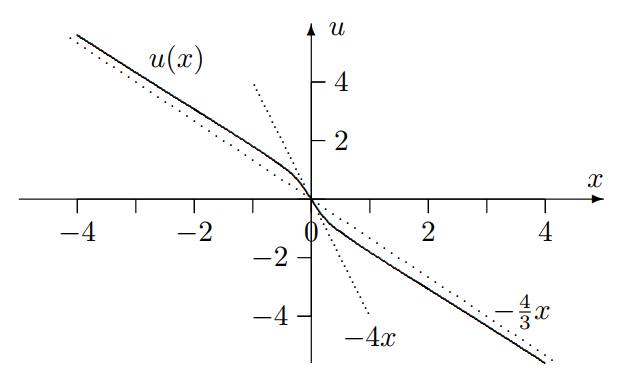
\includegraphics[scale=.8]{hinh2ct.png}
	\caption{Luật điều khiển phi tuyến tối ưu}
\end{figure}\\\\
Các đầu đọc nghiêng (the inclined reader is invited) được mời để xác minh rằng thay thế $\beta u^4$ trong hàm chi phí $\beta u^{2k}$ với $k \geq 2$ dẫn đến kết quả là mức tăng trưởng lớn $$u\approx -\frac{2ka}{(2k-1)b}x$$

\section{Xấp xỉ điều khiển tối ưu}
Trong hầu hết các trường hợp, không tìm thấy giải pháp phân tích nào của phương trình vi phân từng phần Hamilton-Jacobi-Bellman. Hơn nữa, việc giải quyết nó bằng số có thể cực kỳ cồng kềnh.\\\\
Do đó, một phương pháp được trình bày ở đây cho phép tìm các kết quả gần đúng cho luật kiểm soát phản hồi trạng thái cho một vấn đề kiểm soát tối ưu bất biến theo thời gian với không gian vô hạn.\\\\ Chúng ta hãy xem xét một vấn đề kiểm soát tối ưu bất biến theo thời gian với một không gian vô hạn cho một hệ động lực phi tuyến với hàm chi phí không bậc hai, được cấu trúc như sau: \\\\ Tìm một luật điều khiển phản hồi trạng thái tối ưu bất biến theo thời gian $u$: $R^n \to R^m$, sao cho hệ thống động $$\dot{x}(t) = F(x(t), u(t)) = Ax(t) + Bu(t) + f(x(t), u(t))$$ được chuyển từ trạng thái ban đầu $x(0) = x_a$ sang trạng thái cân bằng x = 0 tại thời điểm cuối cùng vô hạn sao cho hàm chi phí \begin{eqnarray}
	J(u) &=& \int_{0}^{\infty}L(x(t), u(t))dt \nonumber \\
	&=& \int_{0}^{\infty}\Big(\frac{1}{2}x^T(t)Qx(t) + x^T(t)Nu(t) + \frac{1}{2}u^T(t)Ru(t) + \ell(x(t), u(t)) \Big)dt \nonumber 
\end{eqnarray} đạt giá trị nhỏ nhất.
Trong vấn đề này, người ta cho rằng các điều kiện sau được thỏa mãn: \begin{itemize}
	\item $[A, B]$ cố định
	\item R > 0
	\item $Q = C^TC \geq$ 0
	\item $[A, C]$ có thể tìm được
	\item $\begin{bmatrix}
	Q&N\\N^T&R
	\end{bmatrix} \geq 0$
	\item $f(x, u)$ chỉ chứa các bậc hai hoặc cao hơn trong $x$ và/hoặc $u$
	\item $\ell(x, u)$ chỉ chứa các bậc hai hoặc cao hơn trong $x$ và/hoặc $u$.
\end{itemize}
\subsection{Ký hiệu}
\subsubsection{Phép toán vi phân} Đối với ma trận Jacobi của các đạo hàm riêng của hàm có giá trị $n$-vectơ $f$ đối với $m$-vector $u$, ký hiệu sau được sử dụng: $$f_u = \frac{\partial f}{\partial u} = \begin{bmatrix}
\frac{\partial f_1}{\partial u_1} & \cdots & \frac{\partial f_1}{\partial u_m}\\ \vdots && \vdots \\ \frac{\partial f_n}{\partial u_1} &\cdots& \frac{\partial f_n}{\partial u_m}
\end{bmatrix}$$
Chú ý rằng kết quả của một vector hàng là đạo hàm vô hướng của hàm $f$.
\subsubsection{Sorting Powers (Phân loại theo lũy thừa (?))} Trong các hàm đa thức, chúng ta tổng hợp các thuật ngữ có cùng công suất (the same power) như sau: \begin{eqnarray}
	f(x, u) &=& f^{(2)}(x, u) + f^{(3)}(x, u) + f^{(4)}(x, u)\cdots \nonumber \\
	\ell(x, u) &=& \ell^{(3)}(x, u) + \ell^{(4)}(x, u) + \ell^{(5)}(x, u) + \cdots \nonumber \\
	T(x) &=& T^{(2)}(x) + T^{(3)}(x) + T^{(4)}(x) + \cdots \nonumber \\ u^o(x) &=& u^{o(1)}(x) + u^{o(2)}(x) + u^{o(3)}(x) + \cdots \nonumber .
\end{eqnarray}
Ví dụ: Trong trường hợp đơn giản nhất của hàm vô hướng với các đối số vô hướng $x$ và $u$, hàm $\ell^{(3)}(x, u)$ có dạng tổng quát sau: $$\ell^{(3)}(x, u) = \alpha x^3 + \beta x^2u + \gamma xu^2 + \delta u^3$$
Đối với các đạo hàm của hàm $f$ và $\ell$, các lũy thừa được sắp xếp theo cách tương tự, ví dụ: \begin{eqnarray}
	f_u(x, u) &=& f_u^{(1)}(x, u) + f_u^{(2)}(x, u) + f_u^{(3)}(x, u) + \cdots \nonumber \\ \ell_u(x, u) &=& \ell_u^{(2)}(x, u) + \ell_u^{(3)}(x, u) + \ell_u^{(4)}(x, u) + \cdots \nonumber
\end{eqnarray}
Lưu ý thực tế sau đây cho đạo hàm của hàm đối với đối số có giá trị vô hướng hoặc giá trị véc tơ: $$\ell_u^{(k)}(x, u) = \frac{\partial\ell^{(k+1)}(x, u)}{\partial u}.$$
Trong ví dụ trước, chúng ta nhận được
$$\ell_u^{(2)}(x, u) = \frac{\partial\ell^{(3)}(x, u)}{\partial u} = \beta x^2 + 2\gamma xu + 3\delta u^2.$$ Từ bây giờ, chúng ta viết $$T_x(x) = T_x^{[2]}(x) + T_x^{[3]}(x) + T_x^{[4]}(x) + \cdots$$ thay vì $T_x^{(1)}(x) + T_x^{(2)}(x) + T_x^{(3)}(x) + \cdots$
Nói chung, loại ký hiệu này sẽ được sử dụng trong phần tiếp theo. 
\subsection{Phương pháp Lukes} Trong bước xấp xỉ đầu tiên, điều khiển tuyến tính $u^o(1)$ được xác định bằng cách giải bài toán điều chỉnh LQ cho hệ động lực tuyến tính và cho phần thuần phương trình bậc 2 của hàm chi phí. \\\\ Trong mỗi bước xấp xỉ bổ sung của phương pháp đệ quy Lukes, một số lũy thừa bổ sung được thêm vào luật phản hồi $u(x)$, trong khi một số lũy thừa bổ sung của xấp xỉ $f$ và $A$ được xử lý.\\\\ Như đã trình bày trong 2.2.4, hai phương trình sau phải được giải gần đúng trong mỗi bước xấp xỉ: \begin{eqnarray}
	H &=& T_x(x)F(x, u) + L(x, u) = 0\\ H_u &=& T_x(x)F_u(x, u) + L_u(x, u)
\end{eqnarray} Trong bài toán sắp tới, chúng ta có các phương trình sau: \begin{eqnarray}
	H &=&T_x(x)[Ax+Bu+f(x, u)] + \frac{1}{2}x^TQx + x^TNu \nonumber\\ && + \frac{1}{2}u^TRu + \ell(x, u) = 0\\ H_u &=& T_x(x)(B + f_u(x, u)) + x^TN + u^TR + \ell_u(x, u) = 0
\end{eqnarray}
Giải phương trình (2.4) với $u^o$: \begin{equation}
	u^{oT} = -[T_x(x)(B + f_u(x, u^o)) + x^TN + \ell_u(x, u^o)]R^{-1}
\end{equation}
\subsubsection{1$^\text{st}$ Approximation: LQ-Regulator} \begin{eqnarray}
	\dot{x}(t) &=& Ax + Bu \nonumber \\
	J(u) &=& \int_{0}^{\infty}\bigg(\frac{1}{2}x^TQx + x^TNu + \frac{1}{2}u^TRu\bigg)dt \nonumber \\ u^{o(1)} &=& Gx \text{ với } G = -R^{-1}(B^TK + N^T), \nonumber
\end{eqnarray} trong đó $K$ là nghiệm duy nhất duy nhất của phương trình Riccati $$[A-BR^{-1}N^T]^TK + K[A-BR^{-1}N^T] - KBR^{-1}B^TK + Q - NR^{-1}N^T = 0$$ Kết quả của hệ điều khiển tuyến tính được mô tả bởi phương trình vi phân $$\dot{x}(t) = [A + BG]x(t) = A^ox(t)$$ và có giá trị hàm chi phí $$T^{(2)}(x) = \frac{1}{2}x^TKx \text{ với } T_x^{[2]}(x) = x^TK.$$
\subsubsection{2$^\text{nd}$ Approximation}
\begin{eqnarray}
	u^o(x) &=& u^{o(1)}(x) + u^{0(2)}(x)\nonumber \\ T_x(x) &=& T_x^{[2]}(x) + T_x^{[3]}(x) \nonumber
\end{eqnarray}
\begin{itemize}
	\item[\textbf{a)}] Xác định $T_x^{[3]}(x)$: \\ Sử dụng (2.3): \begin{eqnarray}
		0 &=& (T_x^{[2]} + T_x^{[3]})[Ax + B(u^{o(1)} + u^{o(2)}) + f(x, u^{o(1)} + u^{o(2)})] \nonumber \\ && + \text{ } \frac{1}{2}x^TQx + x^TN(u^{o(1)} + u^{o(2)}) + \frac{1}{2}(u^{o(1)} + u^{o(2)})^TR(u^{o(1)} + u^{o(2)}) \nonumber \\ && +\text{ } \ell(x, u^{o(1)} + u^{o(2)}) \nonumber
	\end{eqnarray} Thuật ngữ khối: \begin{eqnarray}
		0 &=& T_x^{[3]}[Ax+Bu^{o(1)}] + T_x^{[2]}[Bu^{o(2)}+f^{(2)}(x, u^{o(1)})] \nonumber \\ && + \text{ } x^TNu^{o(2)} + \frac{1}{2}u^{o(1)^T}Ru^{o(2)} + \frac{1}{2}u^{o(2)^T}Ru^{o(1)} + \ell^{(3)}(x, u^{o(1)}) \nonumber \\ &=& T_x^{[3]}A^ox + T_x^{[2]}f^{(2)}(x, u^{o(1)}) + \ell^{(3)}(x, u^{o(1)}) \nonumber \\ && + \text{ } \underbrace{[T_x^{[2]}B + x^TN + u^{o(1)^T}R]}_{= \text{ } 0}u^{o(2)} \nonumber
	\end{eqnarray}
	 Vì vậy, phương trình dành cho $T_x^{(3)}(x)$ là \begin{equation}
	 	0 = T_x^{[3]}A^ox + T_x^{[2]}f^{(2)}(x, u^{o(1)}) + \ell^{(3)}(x, u^{o(1)}).
	 \end{equation}
\item[\textbf{b)}] Xác định $u^{o(2)}(x)$:\\
Sử dụng (2.5): \begin{eqnarray}
	(u^{o(1)} + u^{o(2)})^T = &-& \Big[(T_x^{[2]} + T_x^{[3]})(B+f_u(x, u^{o(1)} + u^{o(2)}) \nonumber \\ && + \text{ } x^TN + \ell_u(x, u^{o(1)} + u^{o(2)})\Big]R^{-1} \nonumber
\end{eqnarray}
Dạng bậc hai: \begin{equation}
	u^{o(2)^T} = - \Big[T_x^{[3]}B + T_x^{[2]}f_u^{(1)}(x, u^{o(1)}) + \ell_u^{(2)}(x, u^{o(1)})\Big]R^{-1}
\end{equation}
\end{itemize}
Chú ý rằng trong hai phương trình (2.6) và (2.7), $u^{o(2)}$ không tồn tại ở vế phải. Do đó đây là các phương trình với hai vế được tách rời. Phương trình (2.7) là phương trình xác định $u^{o(2)}$ - Bước này xuất hiện theo cách tương tự trong các bước xấp xỉ tiếp theo. 

\subsubsection{$3^{\text{rd}}$ Approximation}
\begin{eqnarray}
	u^*(x) &=& u^{o(1)}(x) + u^{o(2)}(x) \nonumber \\ u^o(x) &=&u^*(x) + u^{o(3)}(x) \nonumber \\ T_x(x) &=& T_x^{[2]}(x) + T_x^{[3]}(x) + T_x^{[4]}(x) \nonumber
\end{eqnarray}
\begin{itemize}
	\item[\textbf{a)}] Xác định $T_x^{[4]}(x)$: \begin{eqnarray}
		0 &=& T_x^{[4]}A^ox + T_x^{[3]}Bu^{o(2)} \nonumber \\ && + \text{ }T_x^{[3]}f^{(2)}(x, u^*) + T_x^{[2]}f^{(3)}(x, u^*) \nonumber \\ && \text{ } + \frac{1}{2}u^{o(2)^T}Ru^{o(2)} + \ell^{(4)}(x, u^*) \nonumber
	\end{eqnarray}
	\item[\textbf{b)}] Xác định $u^{o(3)}$: $$u^{o(3)^T} = -[T_x^{[4]}B + T_x^{[3]}f_u^{(1)}(x, u^*) + T_x^{[2]}f_u^{[2]}(x, u^*) + \ell_u^{(3)}(x, u^*)]R^{-1}$$
\end{itemize}
\subsubsection{\textit{k}$^{\text{th}}$ Approximation (\textit{k} $\geq$ 4)}
\begin{eqnarray}
	u^*(x) &=& \sum_{i=1}^{k-1}u^{o(i)} \nonumber\\ u^{o}(x) &=& u^*(x) + u^{o(k)}(x) \nonumber\\ T_x(x) &=& \sum_{j=2}^{k+1}T_x^{[j]}(x) \nonumber
\end{eqnarray}
\begin{itemize}
	\item[\textbf{a)}] Xác định $T_x^{[k+1]}(x)$:\\\\Với $k$ chẵn:
 \begin{equation}
	\begin{split}
	 0 = T_x^{[k+1]}A^ox + \sum_{j=2}^{k-1}T_x^{[k+2-j]}Bu^{o(j)} + \sum_{j=2}^{k}T_x^{[k+2-j]}f^{(j)}(x, u^*) \\+ \sum_{j=2}^{\frac{k}{2}}u^{o(j)^T}Ru^{o(k+1-j)} + \ell^{(k+1)}(x, u^*)
	\end{split} \nonumber
	\end{equation} Với $k$ lẻ:
	\begin{equation}
	\begin{split}
	0 = T_x^{[k+1]}A^ox + \sum_{j=2}^{k-1}T_x^{[k+2-j]}Bu^{o(j)} + \sum_{j=2}^{k}T_x^{[k+2-j]}f^{(j)}(x, u^*) \\ + \sum_{j=2}^{\frac{k-1}{2}}u^{o(j)^T}Ru^{o(k+1-j)} + \frac{1}{2}
		u^{o(\frac{k+1}{2})^T}Ru^{o(\frac{k+1}{2})} + \ell^{(k+1)}(x, u^*) 		
		\end{split} \nonumber
		\end{equation}
	\item[\textbf{b)}] Xác định $u^{o(k)}$: $$u^{o(k)^T} = - \Big[T_x^{[k+1]}B + \ell_u^{(k)}(x, u^*) + \sum_{j=1}^{k-1}T_x^{[k+1-j]}f_u^{(j)}(x, u^*)\Big]R^{-1}$$
\end{itemize}
Các công thức này được thỏa mãn với mọi $k \geq 2$ nếu giá trị của một tổng trống bằng 0.
\subsection{Bộ điều khiển với đặc tính lũy tiến}
Đối với hệ động lực bất biến theo thời gian tuyến tính theo thứ tự đầu tiên, chúng ta muốn thiết kế một điều khiển phản hồi trạng thái bất biến theo thời gian $u(x)$, đặc tính của nó là siêu tuyến tính, tức là $u(x)$ là lũy tiến cho các giá trị lớn hơn của trạng thái $x$.\\\\Để đạt được mục tiêu này, chúng ta xây dựng một hàm chi phí với mục đích kiểm soát theo phương trình bậc hai và trạng thái siêu bậc hai. \\\\
Ví dụ, chúng ta hãy xem xét vấn đề kiểm soát phản hồi trạng thái tối ưu được mô tả bởi các phương trình sau: \begin{eqnarray}
	\dot{x}(t) &=& ax(t) + u(t) \nonumber \\ J(u) &=& \int_{0}^{\infty}\Big(q\cosh(x(t))-q+\frac{1}{2}u^2(t)\Big)dt, \nonumber
\end{eqnarray} trong đó $a$ và $q$ là hằng số dương. \\\\ Sử dụng mở rộng chuỗi $$\cosh(x) = 1 + \frac{x^2}{2!} + \frac{x^4}{4!} + \frac{x^6}{6!} + \frac{x^8}{8!} + \cdots$$ đối với hàm cosin hyperbol, chúng ta có các tương ứng sau với danh pháp được sử dụng trong mục 2.3.2: \begin{eqnarray}
	A&=&a \nonumber\\B&=&1\nonumber\\f(x, u)&\equiv& 0 \nonumber \\ f_u(x, u)&\equiv& 0 \nonumber \\ R&=&1\nonumber\\N&=&0 \nonumber\\Q&=&q\nonumber\\\ell(x, u)&=&q\Big(\frac{x^4}{4!} + \frac{x^6}{6!}+\frac{x^8}{8!} + \cdots\Big) \nonumber\\\ell_u(x, u) &\equiv&0 \nonumber.
\end{eqnarray}
\subsubsection{\textbf{1}$^{\text{st}}$Approximation: LQ-Regulator} \begin{eqnarray}
	\dot{x}&=&ax + u \nonumber\\J(u)&=&\int_{0}^{\infty}\Big(\frac{1}{2}qx^2 + \frac{1}{2}u^2\Big)dt \nonumber\\u^{o(1)}&=&-Kx, \nonumber
\end{eqnarray} với $$K = a + \sqrt{a^2+q}$$ là nghiệm dương của phương trình Riccati $$K^2 - 2aK - q = 0.$$ Kết quả của hệ thống điều khiển tuyến tính được mô tả bởi phương trình vi phân $$\dot{x}(t) = [a - K]x(t) = A^ox(t) = -\sqrt{a^2+q}x(t)$$ và có hàm chi phí $$T^{(2)}(x) = \frac{1}{2}Kx^2 = \frac{1}{2}\Big(a+\sqrt{a^2+q}\Big)x^2$$ với đạo hàm $$T_x^{[2]}(x) = Kx = \Big(a + \sqrt{a^2+q}\Big)x.$$
\subsubsection{\textbf{2}$^{\text{nd}}$ Approximation} 
Từ $$0 = T_x^{[3]}A^ox + T_x^{[2]}f^{(2)} + \ell^{(3)}$$ chúng ta nhận được $$T_x^{[3]} = 0.$$ Vì $f_u(x, u) \equiv 0, \ell_u(x, u) \equiv 0, B=1$ và $R = 1$, chúng ta thu được kết quả sau đây với $k \geq 2$: $$u^{o(k)} = -T_x^{[k+1]}.$$ Vì thế, $$u^{o(2)} = -T_x^{[3]} = 0.$$
\subsubsection{\textbf{3}$^{\text{rd}}$ Approximation}
\begin{align}
	0 = T_x^{[4]}A^ox + T_x^{[3]}Bu^{o(2)} + \sum_{j=2}^{3}T_x^{[5-j]}f^{(j)} + \frac{1}{2}u^{o(2)^T}Ru^{o(2)} + \ell^{(4)} \nonumber \\ T_x^{[4]} = \frac{qx^3}{4!\sqrt{a^2 + q}} \nonumber \\ u^{o(3)} = -T_x^{[4]} = -\frac{qx^3}{4!\sqrt{a^2+q}} \nonumber
\end{align}
\subsubsection{\textbf{4}$^{\text{th}}$ Approximation}
\begin{align}
	0=T_x^{[5]}A^ox + \sum_{j=2}^{3}T_x^{[6-j]}Bu^{o(j)} + \sum_{j=2}^{4}T_x^{[6-j]}f^{(j)} + \sum_{j=2}^{2}u^{o(j)}Ru^{o(5-j)} + \ell^{(5)} \nonumber \\ T_x^{[5]} = 0 \nonumber \\ u^{o(4)} = -T_x^{[5]} = 0 \nonumber
\end{align}
\subsubsection{\textbf{5}$^{\text{th}}$ Approximation}
\begin{align}
	0 = T_x^{[6]}A^ox + \sum_{j=2}^{4}T_x^{[7-j]}Bu^{o(j)} + \sum_{j=2}^{5}T_x^{[7-j]}f^{(j)}  +\sum_{j=2}^{2}u^{o(j)}Ru^{o(6-j)} + \frac{1}{2}u^{o(3)}Ru^{o(3)}+\ell^{(6)} \nonumber \\ T_x^{[6]} = \Big(\frac{q}{6!} - \frac{q^2}{2(4!)^2(a^2+q)}\Big)\frac{x^5}{a^2+q} \nonumber \\ u^{o(5)} = -T_x^{[6]} = -\Big(\frac{q}{6!} - \frac{q^2}{2(4!)^2(a^2+q)}\Big)\frac{x^5}{a^2+q} \nonumber 
\end{align}
\subsubsection{\textbf{6}$^{\text{th}}$ Approximation}
\begin{align}
	0=T_x^{[7]}A^ox + \sum_{j=2}^{5}T_x^{[8-j]}Bu^{o(j)} + \sum_{j=2}^{6}T_x^{[8-j]}f^{(j)} + \sum_{j=2}^{3}u^{o(j)}Ru^{o(7-j)} + \ell^{(7)} \nonumber \\ T_x^{[7]} = 0 \nonumber \\u^{o(6)} = -T_x^{[7]} = 0 \nonumber
\end{align}
\subsubsection{\textbf{7}$^{\text{th}}$ Approximation}
\begin{align}
	0=T_x^{[8]}A^ox + \sum_{j=2}^{6}T_x^{[9-j]}Bu^{o(j)} + \sum_{j=2}^{7}T_x^{[9-j]}f^{(j)} + \sum_{j=2}^{3}u^{o(j)}Ru^{o(8-j)}+\frac{1}{2}u^{o(4)^T}Ru^{o(4)} + \ell^{(8)} \nonumber \\ T_x^{[8]} = \bigg(\frac{q}{8!} - \Big(\frac{q}{6!}-\frac{q^2}{2(4!)^2(a^2+q)}\Big)\frac{1}{4!(a^2+q)}\bigg)\frac{x^7}{\sqrt{a^2+q}} \nonumber \\ u^{o(7)} = -T_x^{[8]} = -\bigg(\frac{q}{8!} - \Big(\frac{q}{6!}-\frac{q^2}{2(4!)^2(a^2+q)}\Big)\frac{1}{4!(a^2+q)}\bigg)\frac{x^7}{\sqrt{a^2+q}} \nonumber
\end{align}
\textbf{và như thế ...} \\\\Cuối cùng, chúng ta có được điều khiển phi tuyến, tối ưu gần đúng sau $$u^o(x) = u^{o(1)}(x) + u^{o(3)}(x) + u^{o(5)}(x) + u^{o(7)}(x) + \cdots $$ Về mặt thực tế, nó có thể được xấp xỉ bằng phương trình sau: $$u^o(x) \approx -(a+\sqrt{a^2 + q})x - 
\frac{qx^3}{4!\sqrt{a^2+q}} - \frac{qx^5}{6!\sqrt{a^2+q}} - \frac{qx^7}{8!\sqrt{a^2+q}}-\cdots$$ Đặc tính của bộ điều khiển xấp xỉ này bị cắt bớt sau bốn thuật ngữ được hiển thị trong Hình 2.3.
\begin{figure}[h]
	\centering
	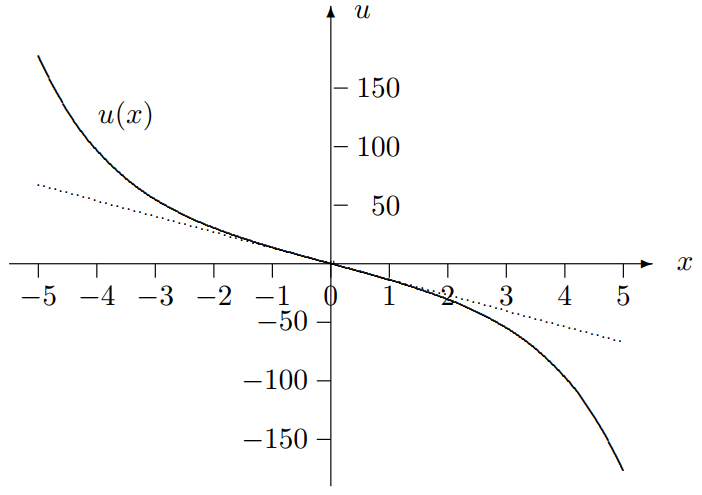
\includegraphics[scale=.6]{hinh5.png}
	\caption{Xấp xỉ điều khiển tối ưu với $a = 3, q = 100$.}
\end{figure}
\subsection{Kiểm soát tốc độ LQQ}
Phương trình chuyển động của vận tốc $v(t)$ của máy bay trong chuyến bay ngang có thể được mô tả bởi $$m\dot{v}(t) = -\frac{1}{2}c_wA_r\rho v^2(t) + F(t) ,$$ Trong đó $F(t)$ là lực đẩy ngang do động cơ phản lực tạo ra, $m$ là khối lượng của máy bay, $c_w$ là hệ số lực cản khí động học, $A_r$ là tiết diện tham chiếu của máy bay và $\rho$ là mật độ của không khí. \\\\Máy bay phải bay với tốc độ không đổi $v_0$. Đối với điều này, lực đẩy danh nghĩa $$F_0 = \frac{1}{2}c_wA_r\rho v_o^2$$ là cần thiết. Chúng ta muốn tăng cường chiến lược điều khiển vòng mở rõ ràng $F(t) \equiv F_0$ bằng điều khiển phản hồi sao cho vận tốc $v(t)$ được kiểm soát chính xác hơn, nếu có bất kỳ sự khác biệt nào xảy ra vì bất kỳ lý do gì. \\\\Giới thiệu biến trạng thái $$x(t) = v(t) - v_0$$ và biến điều khiển phụ hiệu chỉnh $$u(t) = \frac{1}{m}\big(F(t) - F_0\big)$$ các động lực phi tuyến sau đây để thiết kế điều khiển phản hồi thu được: \begin{eqnarray}
	\dot{x}(t) &=& a_1x(t) + a_2x^2(t) + u(t) \nonumber \\ \text{ với } a_1 &=& -\frac{c_wA_r\rho v_0}{m} \nonumber \\ \text{ và } a_2 &=& - \frac{c_wA_r\rho }{2m} \nonumber
\end{eqnarray} Đối với thiết kế của bộ điều khiển phản hồi, chúng ta chọn hàm chi phí bậc hai tiêu chuẩn $$J(u) = \frac{1}{2}\int_{0}^{\infty}\big(qx^2(t) + u^2(t)\big)dt.$$ Do đó, chúng ta có được các tương ứng sau với danh pháp được sử dụng trong Chương 2.3.2: \begin{eqnarray}
	A&=&a_1\nonumber\\B&=&1\nonumber\\f(x, u) &=& a_2x^2 \nonumber \\ f_u(x, y) &\equiv& 0 \nonumber \\ f^{(1)}(x, u) &=& 2a_2x \nonumber \\ f^{(2)}(x, u) &=& 2a_2 \nonumber \\ f^{(3)}(x, u) &=& 0 \nonumber \\ Q&=&q \nonumber \\R&=&1 \nonumber \\\ell(x, u) &\equiv& 0 \nonumber 
\end{eqnarray}
\subsubsection{\textbf{1}$^\text{st}$ Approximation: LQ-Regulator} \begin{eqnarray}
	\dot{x}(t) &=&a_1x + u \nonumber \\ J(u) &=& \int_{0}^{\infty}\Big(\frac{1}{2}qx^2+\frac{1}{2}u^2\Big)dt \nonumber \\ u^{o(1)}&=&-Kx, \nonumber
\end{eqnarray} với $$K = a_1 + \sqrt{a_1^2+q}$$ là nghiệm dương của phương trình Riccati $$K^2-2a_1K-q=0$$ Kết quả của hệ thống điều khiển tuyến tính được mô tả bởi phương trình vi phân $$\dot{x}(t) = [a_1 - K]x(t) = A^ox(t) = -\sqrt{a_1^2+q}x(t)$$ và có hàm chi phí $$T^{(2)}(x) = \frac{1}{2}Kx^2 = \frac{1}{2}\bigg(a_1 + \sqrt{a_1^2+q}\bigg)x^2$$ với đạo hàm $$T_x^{[2]}(x) = Kx = \bigg(a_1 + \sqrt{a_1^2 + q}\bigg)x$$
\subsubsection{\textbf{2}$^\text{nd}$ Approximation}
Từ $$0 = T_x^{[3]}A^ox + T_x^{[2]}f^{(2)} + \ell^{(3)}$$ chúng ta có $$T_x^{[3]} = \frac{a_1 + \sqrt{a_1^2 + q}}{\sqrt{a_1^2 + q}}a_2x^2.$$ Vì $f_u(x, u) \equiv 0, \ell_u(x,u) \equiv 0, B=1$ và $R=1$, chúng ta thu được kết quả sau đây với mọi $k \geq 2$: $$u^{o(k)} = -T_x^{[k+1]}.$$ Vì vậy, $$u^{o(2)} = -T_x^{[3]} = -\frac{a_1+\sqrt{a_1^2+q}}{\sqrt{a_1^2+q}}a_2x^2.$$ Vì phương trình chuyển động là bậc hai theo $x$, thuật toán dừng ở đây. Do đó, luật kiểm soát tối ưu xấp xỉ là: $$u(x) = u^{o(1)}(x) + u^{o(2)}(x) = -\Big(a_1 + \sqrt{a_1^2+q} \Big)x - \frac{a_1 + \sqrt{a_1^2+q}}{\sqrt{a_1^2+q}}a_2x^2.$$ Tính chất của bộ điều khiển xấp xỉ này được hiển thị trong Hình 2.4.
\begin{figure}[h]
	\centering
	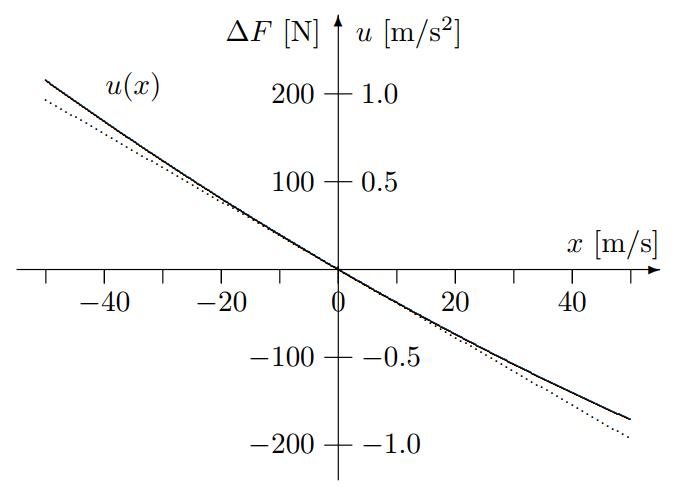
\includegraphics[scale=.6]{hinh6ct.png}
	\caption{Tính chất của điều khiển LQQ với $v_0 = 100$ m/s, $q = 0.001, c_w = 0.05, A_r = 0.5$ m$^2$, $\rho=1.3$kg/m$^3, m = 200$ kg.}
\end{figure}
\end{document} 